\newpage
\section{Installing gpvdm}

\subsection{Windows (if you have admin rights)}
Go to the download page for gpvdm at \url{http://www.gpvdm.com/windows.php} and download the latest version.  Simply double click on it and say yes to all questions.  In general I release a new version every couple of weeks and it's worth keeping your version up-to-date. On modern versions of windows, windows will ask you if you want to install an unsigned executable from an unknown author, and warn you that this could damage your computer.  The reason you get this message is because I have not cryptographically signed the .exe file. I have not signed it because I do not own a private cryptographic key with which to do this.  To get such a key I would have to send my passport off to a key authority to prove who I am and then pay them 500 pounds/year for the privilege of them validating who I am.  Needless to say, that I am not very excited about paying 500 pounds/year so you will just have to click away the warnings from windows.

\subsection{Windows (No admin rights)}
If you don't have admin rights to your computer it can be hard to install new software, gpvdm offers the option of running gpvdm while not properly installed.  Download the zip file containing gpvdm from \url{https://www.gpvdm.com/download_no_admin.php}.  Once you have downloaded the zip archive, open the zip file and extract the folder $pub$ to c:\textbackslash . Then rename the folder to be calledc:\textbackslash gpvdm.  Once you have done this run the executable c:\textbackslash gpvdm\textbackslash gpvdm.exe (see figure \ref{fig:directory}).

\begin{figure}[H]
\centering
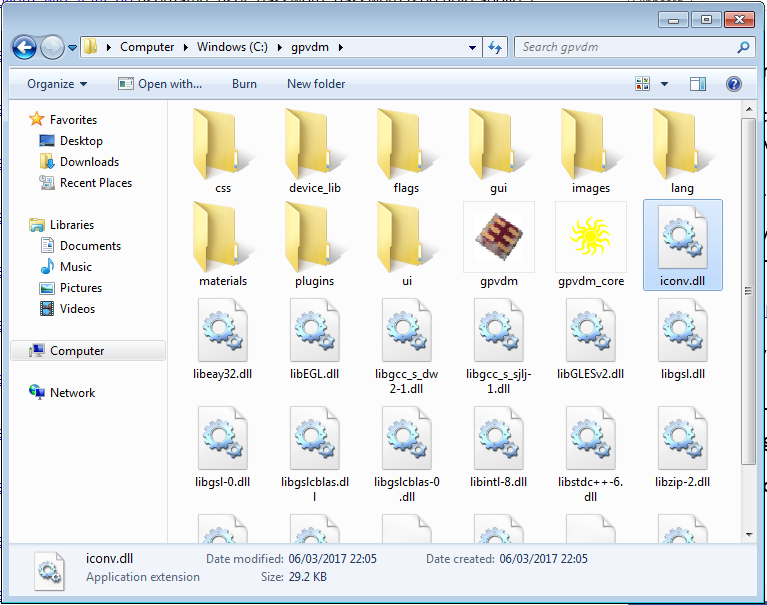
\includegraphics[width=70mm]{./images/dir.png}
\caption{Running and installing gpvdm.  Double click on the gpvdm icon to run the model.}
\label{fig:directory}
\end{figure}

\subsection{Linux} \label{installing_on_linux}
The windows version of gpvdm seems to be much more popular than the Linux version.  Therefore, I will tend to publish an updated windows exe every couple of weeks (along with the platform independent source code) and only publish updated linux rpms/deb packages when someone asks me to.  This means that the Linux deb/rpm files tend to lag behind the windows version by about a year.  For this reason I recommend you install the Linux version from source.


\subsubsection{Linux from source the easy way}
Download the gpvdm by issuing the command

\begin{verbatim}
git clone  https://github.com/roderickmackenzie/gpvdm
\end{verbatim}
Find your operating system in

\begin{verbatim}
build_system/dependency_scripts
\end{verbatim}

This script should install all the packages you need to run/compile gpvdm for a given OS. I don't always keep them up to date, so if you have a new version of an OS and the packages have been renamed you may have to hunt around.

Then run:
\begin{verbatim}
./build
\end{verbatim}

Then select, (compile), and (auto). Then hit return to build.


\begin{figure}[H]
\centering
\includegraphics[width=0.7\textwidth]{./images/build.png}
\caption{The linux build system, run ./build to get this menu.  }
\label{fig:build}
\end{figure}



